%%%%%%%%%%%%% Configuración %%%%%%%%%%%%%%%%%%%%%%



\documentclass[12pt,a4paper,spanish]{book}

\usepackage{amsmath,amssymb,amsfonts,mathrsfs}
\usepackage{graphicx}
\usepackage{anysize}
\usepackage[utf8]{inputenc}
%\usepackage[english]{babel}
%\usepackage[latin1]{inputenc}
\usepackage[spanish]{babel}  %Quita el comentario a esta línea y comenta la siguiente si quieres que los números romanos aparezcan en mayúsculas
%\usepackage[spanish, es-lcroman]{babel} 
\usepackage[bf]{caption}
\usepackage{subfigure}
\usepackage{rotating}
\usepackage{fontenc}
%\usepackage{mathaccent}
\usepackage{titlesec}
\usepackage{multirow} %Para poder centrar verticalmente el contenido de las celdas de una tabla
\usepackage{fancyhdr} %Para personalizar los encabezados y pies de página
\usepackage{acronym}  %Para expandir automáticamente los acrónimos
\usepackage[titletoc]{appendix} %Para que cambie el título y la forma de numerar los apéndices


%Define el formato de los encabezados y pies de página del índice y la lista de acrónimos
\fancypagestyle{plain}{ %Encabezado y pie para el índice y acrónimos
 \fancyhf{}  %Elimina encabezdo y pie (menos la línea del encabezado)
 \renewcommand{\headrulewidth}{0pt} %Elimina la línea del encabezado
 \fancyfoot[LE,RO]{\thepage}
}


\marginsize{2.5cm}{2.5cm}{2.5cm}{2.5cm}

\linespread{1.5}

% Esto es para redefinir los títulos que Latex pone por defecto
\addto\captionsspanish{\renewcommand{\contentsname}{Contenido}}
\renewcommand{\tablename}{Tabla}

%Esto es para redefinir el formato en que se presenta el título de los capítulos
\titleformat{\chapter}[hang]{\Huge\bfseries}{\fontsize{24}{60} Capítulo \thechapter{. }}{0pt}{\fontsize{24}{60}}


\newcommand{\reff}[1]{Figura \ref{#1}}
\newcommand{\refe}[1]{(\ref{#1})}
\renewcommand{\captionfont}{\small}

%Si el idioma es español las listas aparecen con un cuadradito.
%En inglés aparecen con un bullet...Esto redefine el bullet a cuadrado.
\renewcommand{\labelitemi}{\tiny{$^\blacksquare$}}

%\renewcommand{\figurename}{Fig.}

\hyphenation{mo-du-la-tion pa-ra-me-te-ri-zed res-pon-se cha-rac-ter par-ti-cu-la-ri-zing de-ve-lo-ped a-ve-ra-ging pro-ba-bi-li-ty me-cha-nism par-ti-cu-lar know-led-ge pro-ducts inter-operable to-po-lo-gy cha-rac-te-ri-zed stra-te-gy rea-li-za-da si-mu-la-cio-nes pro-pues-tas pro-pues-to cen-tra-li-za-das igua-la-do-res su-mi-nis-tro va-lo-ra-do in-ter-fe-ren-cia par-ti-cu-la-ri-ties mul-ti-plexing ins-ti-tu-te ca-rri-er maxi-mum carre-te-ras} %es un modo burdo de definir como romper una palabra

%\sloppy %permite que sea permisivo con las líneas sueltas


%%Para que las viñetas del segundo nivel aparezcan como a),b)...y no (a), (b)
\renewcommand{\theenumii}{\alph{enumii}}
\renewcommand{\labelenumii}{\textsf{\theenumii})}

%Para las url en la bibliografía
\usepackage{url}

%Para escribir codigo
\usepackage{listings}

\usepackage{color}
\usepackage{listings}
\lstset{ %
language=C++,                % choose the language of the code
basicstyle=\footnotesize,       % the size of the fonts that are used for the code
%numbers=left,                   % where to put the line-numbers
%numberstyle=\footnotesize,      % the size of the fonts that are used for the line-numbers
%stepnumber=1,                   % the step between two line-numbers. If it is 1 each line will be numbered
%numbersep=5pt,                  % how far the line-numbers are from the code
backgroundcolor=\color{white},  % choose the background color. You must add \usepackage{color}
showspaces=false,               % show spaces adding particular underscores
showstringspaces=false,         % underline spaces within strings
showtabs=false,                 % show tabs within strings adding particular underscores
%frame=single,           % adds a frame around the code
tabsize=2,          % sets default tabsize to 2 spaces
captionpos=b,           % sets the caption-position to bottom
breaklines=true,        % sets automatic line breaking
breakatwhitespace=true,    % sets if automatic breaks should only happen at whitespace
escapeinside={\%*}{*)}          % if you want to add a comment within your code
}




 
%El fichero config.tex contiene:
% \input{config.tex}: Define los parámeros comunes a todo el documento (tipo de letra, tamaño,  %márgenes, etc.). También se incluyen los paquetes que el compilador necesita para manejar %cosas "extrañas" como las figuras o el español en lugar del inglés!

%%%%%%%%%%%%%%%%%%%%%%%%%%%%%%%%%%%%%%%%%%%%%%%%%%%%%%%%%%%%%%%%%%%%%%%%%%%%%%%%%%%%%%%%%%%%%%%%%%%%%%
%%%%%%%%%%%%%%%%%%%%%%%%%%%%%%%%%%%%%%%%% COMIENZA EL DOCUMENTO
%%%%%%%%%%%%%%%%%%%%%%%%%%%%%%%%%%%%%%%%%%%%%%%%%%%%%%%%%%%%%%%%%%%%%%%%%%%%%%%%%%%%%%%%%%%%%%%%%%%%%%
\begin{document}
\parindent 0cm  %elimina el indentado de párrafos
\pagestyle{empty}  %Para que no numere ni ponga encabezado ni los agradecimientos ni la dedicatoria

%%%%%%%%%%%%%%%%%%%%%%%%%%%%%%%%%%%%%%%%%%%%
% Agradecimientos
%%%%%%%%%%%%%%%%%%%%%%%%%%%%%%%%%%%%%%%%%%%%
%\emph{ }

\vspace{7mm}
\textbf{\huge{Agradecimientos}}
\vspace{2mm}

Aquí se colocan los agradecimientos. 

\cleardoublepage

  %Aquí van los agradecimientos

%%%%%%%%%%%%%%%%%%%%%%%%%%%%%%%%%%%%%%%%%%%%%
% Dedicatoria
%%%%%%%%%%%%%%%%%%%%%%%%%%%%%%%%%%%%%%%%%%%%
%\begin{flushright}
%\textit{Aquí va la dedicatoria \\
%cada línea se separa por \\}
%\end{flushright}


\cleardoublepage
\pagenumbering{roman}
\pagestyle{plain} %define el formato de la cabecera
\addcontentsline{toc}{chapter}{\hspace{5.26mm}Lista de Acrónimos}
\renewcommand{\contentsname}{Índice}  %Quitar el comentario a esta línea si se quiere que en lugar de "Contenidos" aparezca "índice"
\tableofcontents
\listoffigures

\cleardoublepage


%Inclusión de la lista de acrónimos
%Lista de acrónimos 
\chapter*{Acrónimos}

\begin{acronym}[DLMS/COSEMM]
	\acro{TFG}{Trabajo Fin de Grado}
	\acro{ALPR}{Automatic License Plate Recognition}
	\acused{ALPR}
\end{acronym}


\cleardoublepage
%Cambia el estilo del encabezado
\pagenumbering{arabic}
\pagestyle{fancy}
\setlength{\headheight}{15pt}
\fancyhf{}
\fancyfoot[LE,RO]{\thepage}
\fancyhead[LE,RO]{\nouppercase{\leftmark}}
\renewcommand{\headrulewidth}{0.1pt} %Elimina la línea del encabezado


%Aquí se deben ir incluyendo los ficheros que contienen cada uno de los capítulos y las referencias y apéndices (si los hubiere)
% ------------------------------------------------------------------------
%                             Capítulo 1
% ------------------------------------------------------------------------
\chapter{Introducción}
En las últimas décadas el gran aumento del número de vehículos circulando por las carreteras ha puesto de manifiesto la necesidad de desarrollar nuevas técnicas de gestión de tráfico que permitan la automatización de este proceso.\\

Los sistemas \ac{ALPR} (Automatic License Plate Recognition) son un elemento clave para lograr esta automatización. Ya que permiten identificar un vehículo en distintas situaciones sin ser necesaria la intervención de un operario humano.

\section{Importancia de los sistemas \acs{ALPR}}
Las técnicas \acs{ALPR} consisten en la extracción de la información de la matrícula de un vehículo a través de una imagen o secuencia de imágenes. 

Dichas técnicas juegan un papel importante en numerosas aplicaciones de la vida real, como el cobro automático de peajes, la ayuda a la policía de tráfico, el control de acceso a párquines o la motorización del tráfico en las carreteras. \cite{IEEEtrans}\\

La gran proliferación de los sistemas \ac{ALPR} en los últimos años se debe, en parte, a la evolución de los sistemas empotrados: sistemas de propósito específico con la mayoría de sus componentes integrados en la misma placa de circuito impreso. \cite{ wiki1}

Los sistemas empotrados permiten la implementación de un sistema \acs{ALPR} completo en poco espacio con un coste y consumo reducido. 

\section{Objetivos del \acf{TFG}}
El \ac{TFG} aquí presentado tiene como objetivo el desarrollo de un algoritmo \acs{ALPR} básico con vistas a su implementación en un placa de sistema empotrado Raspberry Pi, equipada con una cámara de vídeo. El desarrollo del algoritmo se realizará mediante el entorno Matlab, para posteriormente portar el algoritmo a C++ haciendo uso de la librería gráfica OpenCV y poder así ejecutarlo en la placa.

\section{Estructura de la memoria}
Esta memoria se ha estructurado en cinco capítulos:
\begin{enumerate}
\item \textbf{Introducción:} Se plantean las motivaciones para la realización de este \ac{TFG} y los objetivos que pretenden alcanzarse.

\item \textbf{Algoritmos y herramientas:} Se presentan algunos de los programas utilizados y los algoritmos esenciales para el trabajo.

\item \textbf{Desarrollo del algoritmo \ac{ALPR}:} En este apartado se describen los pasos seguidos para la creación del algoritmo \ac{ALPR} mediante Matlab.

\item \textbf{Implementación en C++:} Una vez explicado con detalle el algoritmo, este apartado pasa a centrarse en las diferencias y dificultades encontradas en el proceso de portar el código desarrollado en Matlab a C++.

\item \textbf{Conclusiones y líneas futuras:} Se exponen las conclusiones a las que se ha llegado tras la realización del trabajo; así como algunas de las posibles vías de ampliación y mejora del proyecto.
\end{enumerate}

% ------------------------------------------------------------------------
%                             Capítulo 2
% ------------------------------------------------------------------------
\chapter{Algoritmos y herramientas}
En este capítulo se describen los algoritmos y herramientas utilizados para la realización de este \ac{TFG}; así como los principales motivos para su elección.

\section{Matlab}
Para el desarrollo del algoritmo se necesita un entorno de programación que aporte las funciones necesarias de tratamiento de imagen y que, al mismo tiempo, facilite la manipulación y depuración de código. Por ello se ha elegido el entorno Matlab.\\

Dicho entorno ha sido elegido de acuerdo a las siguientes razones:
\begin{itemize}
\item Experiencia previa en el uso del entorno Matlab en distintas asignaturas cursadas durante la carrera.
\item Facilita el tratamiento digital de imagen gracias al gran número de funciones disponibles.
\item Permite la representación de imágenes como matrices, lo que simplifica su tratamiento.
\item Existencia de abundante documentación y una gran comunidad de usuarios.
\end{itemize}

\section{OpenCV 4.8}
Para poder ejecutarlo en la placa Raspberry Pi, necesitamos portar nuestro código desarrollado en Matlab a C++. Dicha tarea requiere el uso de funciones de tratamiento digital de imagen. Para ello, recurrimos a la librería gráfica OpenCV.\\

Entre las razones para la elección de esta librería en particular destacan:
\begin{itemize}
\item Soporte para múltiples plataformas y sistemas operativos, siendo particularmente interesante el soporte para Raspberry Pi y Linux.
\item Incluye todas las funciones necesarias para portar el algoritmo.
\item Es software libre, por lo que está disponible de forma completamente abierta sin licencias privativas.
\item Existencia de abundante documentación y una gran comunidad de usuarios.
\end{itemize}

\section{Algoritmo de detección de contornos}\label{canny}
La detención de contornos es un proceso mediante el cual, a partir de una imagen en escala de grises, obtenemos las zonas dónde se producen fuertes discontinuidades. Dichas discontinuidades generalmente coinciden con los bordes de los objetos retratados por la imagen.

Este procedimiento resulta útil para un gran número de aplicaciones, ya que un mapa de contornos contiene parte significativa de la información almacenada en la imagen, pero con una complejidad mucho menor. \cite{IEEEedge} Un ejemplo de mapa de contornos puede verse en la \reff{contornos}.\\

\begin{figure}[!h]
\centering \subfigure[Original.]{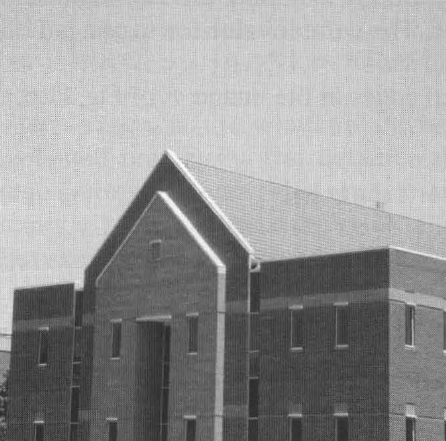
\includegraphics[width=6cm]{Ejem_Cont_Org.png}}
\subfigure[Mapa de contornos.]{
\includegraphics[width=6cm]{Ejem_Cont_Result.png}}
\caption{\small{Efecto del escalado sobre la imagen. Fuente:} \cite{ImgProcessMat}} \label{contornos}
\end{figure}

La figura (a) representa la imagen original en escala de grises, mientras que la figura (b) representa el mapa de contornos obtenido. Como puede apreciarse, la imagen (b) tiene una complejidad menor, ya que sólo contiene información acerca de los bordes de los objetos representados. 

Esta información resulta suficiente para numerosas aplicaciones que traten de localizar objetos dentro de una imagen, como la aplicación \ac{ALPR} que nos ocupa.\\

La idea básica para buscar un mapa de contornos es encontrar las partes de la imagen donde la intensidad cambia rápidamente usando estos dos criterios:

\begin{enumerate}
\item Encontrar las zonas donde la primera derivada es mayor que un determinado umbral.
\item Encontrar las zonas donde la segunda derivada presenta un cruce por cero.
\end{enumerate}


En tratamiento de imagen la primera derivada es el gradiente de una función de dos dimensiones, cuya expresión viene dada por la ecuación:

\begin{equation}
\boldsymbol{\nabla f}= \left[ \begin{array}{c} G_{x} \\ G_{y}  \end{array} \right] =  \left[ \begin{array}{c} \frac{\partial f}{\partial x} \\ \frac{\partial f}{\partial y}  \end{array} \right]
 \label{ecuacion1}
\end{equation}

El algoritmo trabaja con la magnitud de este vector calculada de la siguiente forma:

\begin{equation}
\nabla f=mag( \boldsymbol{\nabla f})=\sqrt{[G_{x}^{2}+G_{x}^{2}]}
\end{equation}

En cuanto a la derivada de segundo orden, normalmente es calculada usando el Laplaciano, como muestra la ecuación:

\begin{equation}
\nabla^{2}f(x,y)=\frac{\partial ^{2} f(x,y)}{\partial x^{2}} + \frac{\partial ^{2} f(x,y)}{\partial y^{2}}
\end{equation}





Existen multitud de algoritmos para detectar los contornos en una imagen. En este \ac{TFG} se han realizado pruebas con dos de los más conocidos: el algoritmo de Canny y el algoritmo de Sobel.

\subsection{Algoritmo de Sobel}
La principal característica del algoritmo de Sobel es que calcula la primera derivada  mediante una aproximación basada en las diferencias entre filas y columnas de los píxeles vecinos en un área de 3X3 como muestra la Ecuación \refe{ecuacion1} y la  \reff{VecinosSobel}.

\begin{figure}[!h]
\centering
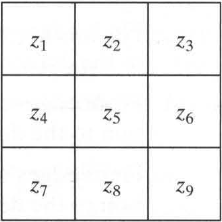
\includegraphics[width=3cm]{VecinosSovel.png}
\caption{\small{Vecinos en el algoritmo de Sobel. Fuente:}\cite{ImgProcessMat}}
\label{VecinosSobel}
\end{figure}

\begin{equation}
g= \sqrt{G_{x}^{2}+G_{x}^{2}}
= \sqrt{[(z_{7} + 2z_{8} + z_{9})-(z_{1} + 2z_{2} + z_{3})]^{2} + (z_{3} + 2z_{6} + z_{9})-(z_{1} + 2z_{4} + z_{7})]^{2} }
\label{ecuacion1}
\end{equation}

Por tanto, decimos que un píxel en una localización determinada (x,y) pertenece a un contorno si g $\geq$ T, siendo T un umbral determinado previamente. \\

En caso de no especificarse el valor del parámetro, el algoritmo lo calcula por sí mismo; siendo ademas posible indicarle una dirección preferente (horizontal o vertical) para buscar los contornos.\\

Se eligió este algoritmo en primer lugar debido a su facilidad de uso, ya que no es necesario ajustar ningún parámetro. El resultado, sin especificar ningún umbral y marcando como dirección preferente la horizontal, se muestra en la \reff{EjemploSobel}.

\begin{figure}[!h]
\centering
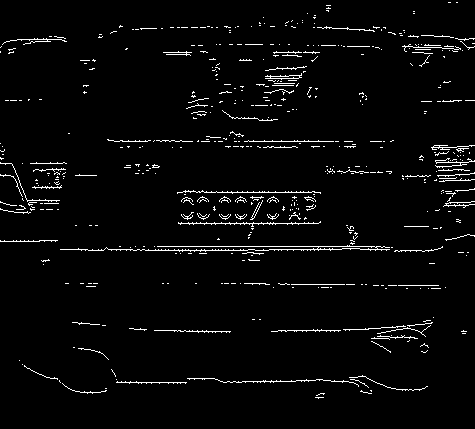
\includegraphics[width=6cm]{EjemploSobel.png}
\caption{\small{Resultado de la detección de ejes con el algoritmo de Sobel.}}
\label{EjemploSobel}
\end{figure}

Como se puede observar en la imagen, el resultado no cumple con las necesidades de la aplicación: aparece mucho ruido en la imagen y las líneas contienen numerosas discontinuidades. 

Para resolver el problema tratado en este \ac{TFG} se necesita un mapa de contornos más simple. Es decir: sólo es necesario que aparezcan los contornos más representativos, que deben estar bien definidos y sin discontinuidades.

\subsection{Algoritmo de Canny}
El algoritmo detector de Canny consta de cuatro pasos:

\begin{enumerate}
\item El ruido de la imagen se reduce mediante el uso de un filtro gaussiano de  desviación típica $\sigma$.

\item Se calcula la primera derivada de la imagen empleando el mismo método que el algoritmo de Sobel.

\item Aplica dos umbrales T1 y T2, siendo T1$<$T2, a la primera derivada calculada anteriormente. Los píxeles para los que el valor es mayor que T2 son llamados píxeles fuertes, mientras que aquellos con un valor entre T1 y T2 son llamados píxeles débiles. A los demás se les fija su valor a 0. Este proceso se conoce como \emph{nonmaximal suppression.}

%\item Los puntos calculados en el apartado anterior dan lugar a picos en el gradiente de la imagen. El algoritmo busca la cima de esos picos y fija a cero todos los píxeles que no pertenecen a ella, conociéndose este proceso como \emph{nonmaximal suppression.} Los píxeles de la cima se determinan mediante dos umbrales T1 y T2, siendo T1$<$T2, los píxeles con un gradiente mayor que T2 son llamados píxeles fuertes y aquellos con un valor entre T1 y T2 son llamados píxeles débiles.

\item Finalmente, el algoritmo forma el contorno incorporando a los píxeles fuertes los píxeles débiles que se encuentren a una distancia de ocho píxeles o menos. 
\end{enumerate}

Se han realizado pruebas con este algoritmo por ser el más potente de los algoritmos de detección de contornos, pero, al contrario que con el algoritmo de Sobel, debemos ajustar los parámetros de la desviación estándar  y los umbrales. El resultado, tras una correcta calibración, se muestra en la \reff{EjemploCanny}\\

\begin{figure}[!h]
\centering

\includegraphics[width=6cm]{EjemploCanny.png}
\caption{\small{Resultado de la detección de ejes con el algoritmo de Canny.}}
\label{EjemploCanny}
\end{figure}

Los resultados son significativamente mejores que los obtenidos con el algoritmo de Sobel. En esta ocasión sólo aparecen los contornos más significativos de la imagen, y las líneas están perfectamente definidas. Por tanto, éste es el algoritmo elegido finalmente para llevar a cabo el detector de matrículas.\\

Para más información sobre los algoritmos de detección de contornos consultar \cite{ImgProcess}.

\section{Transformada de Hough}\label{hough}
Dada una imagen binaria, si queremos encontrar subconjuntos de píxeles que formen líneas rectas, una posible solución es encontrar primero todas las líneas formadas por cada par de píxeles para, posteriormente, buscar todos los píxeles que se encuentren próximos a cada una de la líneas.

El problema de esta solución es que es necesario encontrar $n(n-1)/2 \simeq n^{2}$ líneas así como realizar $n(n(n-1))/2 \simeq n^{3}$ comparaciones entre los n píxeles y todas las líneas. Esta solución resulta computacionalmente irrealizable en cualquier aplicación, excepto en los ejemplos más triviales.\\

Para realizar una aproximación al problema de la detección de líneas rectas que el sistema pueda soportar empleamos la transformada de Hough.\\

Sea un punto $(x_{i},y_{i})$. Las infinitas líneas que pasan a través de él satisfacen la ecuación $y_{i}=ax_{i}+b$. Si se reorganiza la ecuación escribiéndola de la forma $b=-ax_{i}+y_{i}$ y se considera el plano ab\footnote{Plano ortonormal con la variable $b$ en el eje de abscisas y la variable $a$ en el eje de ordenadas}, el punto $(x_{i},y_{i})$ determina de forma inequívoca una recta. Sea otro punto $(x_{j},y_{j})$. Éste determinará otra recta en el plano ab. Dicha recta se cortará con la anterior en el punto $(a' , b')$, siendo $a'$ la pendiente de la recta que determinan los dos puntos en el plano $xy$, y $b'$ el corte de dicha recta con $x=0$. Esta idea queda ilustrada en la  \reff{planoab}. \\

\begin{figure}[!h]
\centering
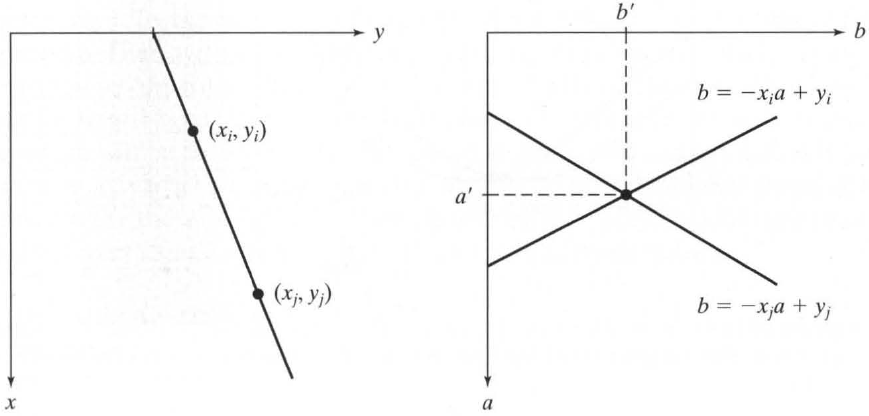
\includegraphics[width=12cm]{planoab.png}
\caption{\small{Relación entre el plano $xy$ y el plano $ab$. Fuente:\cite{ImgProcessMat}}}
\label{planoab}
\end{figure}

De esta forma, usando el plano $ab$ podrían calcularse todas las líneas correspondientes a cada píxel de la imagen; siendo posible determinar las principales líneas rectas simplemente buscando aquellos puntos en el plano $ab$ donde intersecten un gran número de líneas.\\

Una dificultad que presenta esta técnica es que cuando $a$ tiende a infinito, las rectas tienden a ser verticales. Por este motivo, se realiza un cambio a coordenadas esféricas quedando la ecuación, de la recta de la siguiente forma:
\begin{equation}
x \cos{\theta} + y \sin{\theta} = \rho
\end{equation}

Con ésta representación, el plano $ab$ pasa a ser el plano $\theta\rho$; tal y cómo muestra la \reff{planoabesf}. \\

\begin{figure}[!h]
\centering
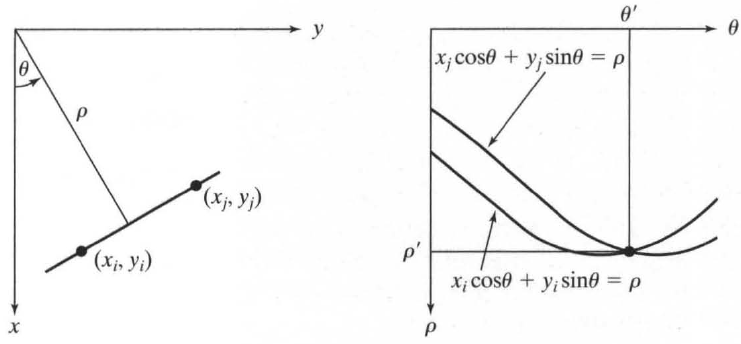
\includegraphics[width=12cm]{planoabesfericas.png}
\caption{\small{Relación entre el plano $xy$ y el plano $ab$ en esféricas. Fuente:\cite{ImgProcessMat}}}
\label{planoabesf}
\end{figure}


Para más información sobre la detección de líneas rectas mediante transformada de Hough consultar \cite{ImgProcess}.
% ------------------------------------------------------------------------
%                             Capítulo 3
% ------------------------------------------------------------------------
\chapter{Desarrollo del algoritmo \acs{ALPR}}
En este capítulo se va a tratar la estructura del algoritmo \ac{ALPR}, así como su desarrollo en el entorno Matlab. 

La tarea que debe realizar este algoritmo es claramente divisible en tres tareas más simples. Primero, se debe encontrar la zona de la imagen donde se encuentra la matrícula. Una vez aislada esa parte de la imagen, se debe extraer cada uno de los dígitos que componen el número de matrícula. Por último, se deben analizar cada uno de los dígitos para determinar con qué carácter se corresponden.

\section{Detección del recuadro de la matrícula}
Para diferenciar el recuadro de la matrícula del resto de la fotografía se han utilizado dos elementos comunes a la mayoría de las matrículas: 
\footnote{Debido a la corta duración del \ac{TFG} el trabajo se centrará exclusivamente en matrículas europeas no compactas.}

\begin{itemize}
\item Un recuadro con unas dimensiones aproximadas conocidas.
\item Letras negras sobre un fondo blanco.
\end{itemize}

El diagrama de flujo del proceso realizado se puede ver en la \reff{diagrecuadro}. A continuación, vamos a analizar en detalle cada una de las fases.

\begin{figure}[!h]
\centering
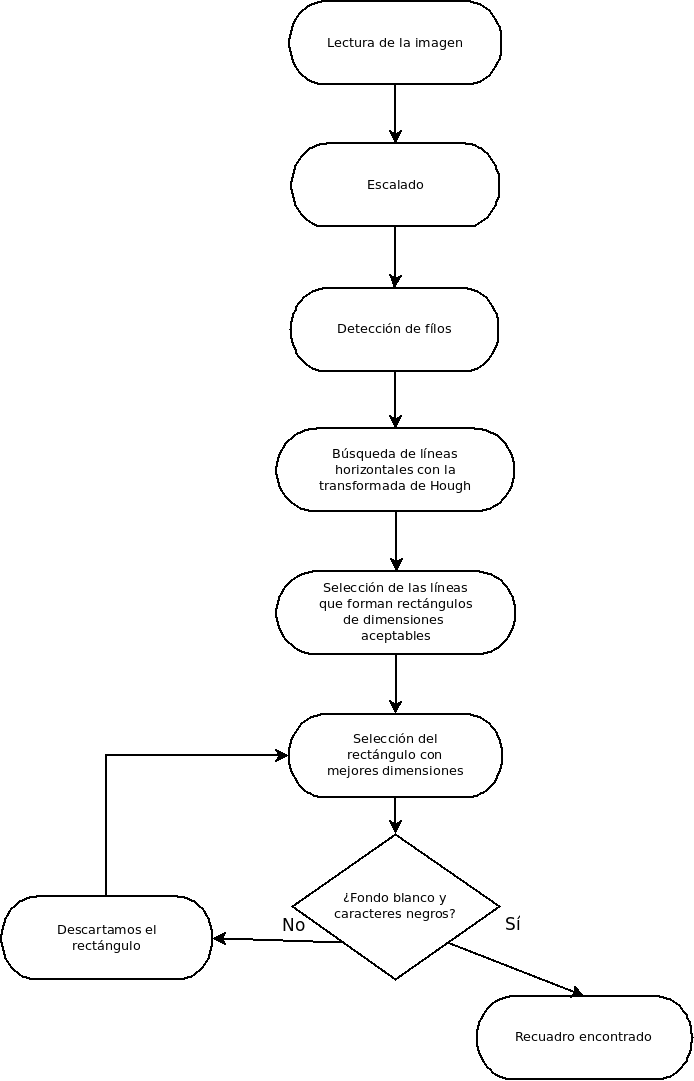
\includegraphics[width=12cm]{DiagramaProyecto.png}
\caption{\small{Diagrama de flujo para la búsqueda del recuadro.}}
\label{diagrecuadro}
\end{figure} 

\subsection{Escalado}
El primer paso consiste en aplicarle un escalado a la imagen, puesto que la cámara de 5 Mpx con la que se ha trabajado tiene demasiada resolución y capta detalles innecesarios que sólo empeoran el resultado. Para esta aplicación se empleará un factor de escalado de tres. El efecto puede verse en la \reff{figescalado}.

\begin{figure}[!h]
\centering \subfigure[Original]{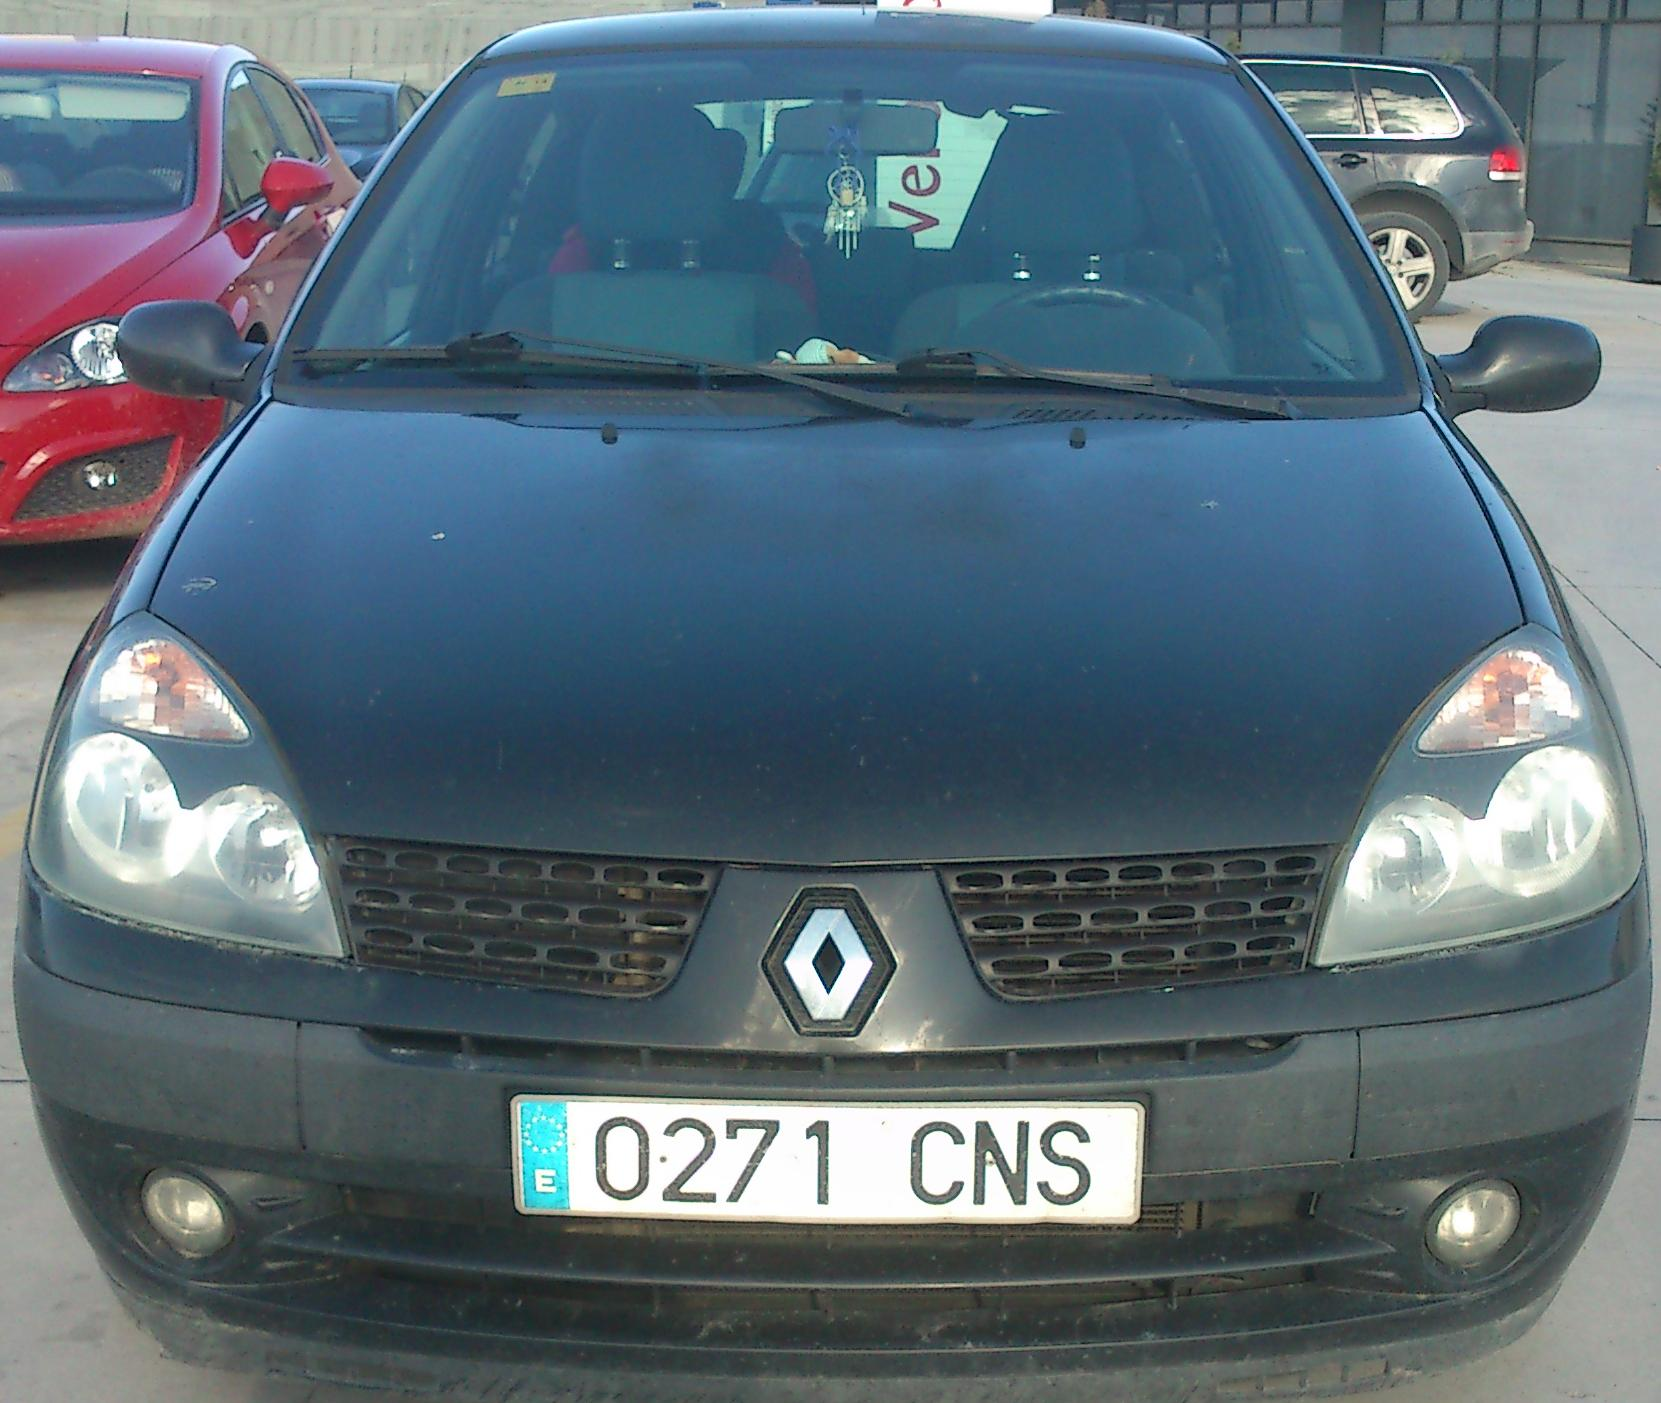
\includegraphics[width=9cm]{Original.png}}
\subfigure[Reducida]{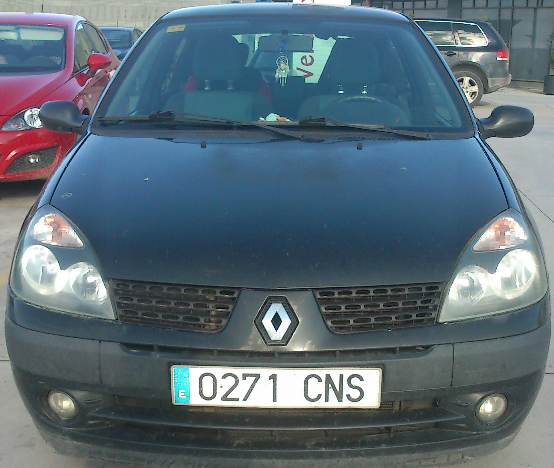
\includegraphics[width=3cm]{Reducida.png}}
\caption{\small{Efecto del escalado sobre la imagen.}} \label{figescalado}
\end{figure}

La reducción del tamaño de la imagen también trae consigo una reducción del tiempo que el algoritmo tarda en procesarla. Esto resulta particularmente importante puesto que el objetivo último de este \ac{TFG} es ejecutar el algoritmo en un sistema empotrado, donde la capacidad de proceso es muy limitada.

\subsection{Detección de contornos}\label{Canny}
La detección de contornos es un paso fundamental para la búsqueda de líneas rectas. Dicho proceso lo llevamos a cabo mediante el algoritmo de Canny. El funcionamiento del mismo y los motivos de su elección ya se trataron en el apartado \ref{canny}.\\

En Matlab se implementa mediante la función

\begin{lstlisting}
edge(Img, canny', [T1,T2], sigma);
\end{lstlisting}

\newpage 
Donde:
\begin{itemize}
\item \textbf{T1 y T2} se corresponden con los umbrales usados por el algoritmo para determinar los contornos. En esta aplicación se ha elegido [\emph{T}1 , \emph{T}2]=[0.12 ,  0.3].

\item \textbf{sigma} es la desviación típica del filtro gaussiano utilizado por el algoritmo para eliminar el ruido de la imagen. En este caso se empleará $sigma=3$.
\end{itemize}

La elección de los valores finales se ha realizado a partir de pruebas sobre distintas imágenes con diferentes condiciones de luminosidad y color; buscando reducir al máximo los detalles de la imagen sin perder las líneas que marcan la placa de matrícula. Los valores por los que finalmente se ha optado son aquellos que mejores resultados han dado en las situaciones de buena luminosidad.\footnote{Se entiende por buena luminosidad una luminosidad uniforme y sin destellos en la parte de la matrícula.}\\

El resultado del algoritmo con los parámetros finales se muestra en la \reff{Cannyfinal}


\begin{figure}[!h]
\centering

\includegraphics[width=6cm]{EjemploCanny.png}
\caption{\small{Efecto de la función Canny con los parámetros seleccionados.}}
\label{Cannyfinal}
\end{figure}

A continuación, se analizará el efecto que produce sobre los resultados la variación de estos parámetros.\\

Los umbrales \textbf {T} definen cómo de brusca ha de ser la discontinuidad en la intensidad de la imagen. Un valor demasiado pequeño resultaría en un excesivo número de contornos, lo que dificultaría la elección de los contornos que forman la matrícula; mientras que un valor demasiado grande provocaría que las líneas de la matrícula no fueran detectadas.  El efecto de los cambios sobre este parámetro puede observarse en la \reff{CannyT}.

\begin{figure}[!h]
\centering \subfigure[Umbral Bajo.]{
\includegraphics[width=6cm]{Tbajo.png}}
\subfigure[Umbral Alto.]{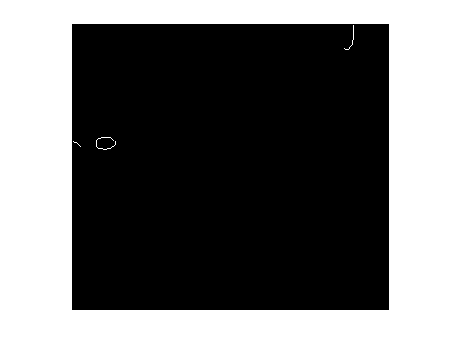
\includegraphics[width=6cm]{Talto.png}}
\caption{\small{Efecto de la modificación del parámetro T.}} \label{CannyT}
\end{figure} 

En la imagen (a) se define un umbral demasiado bajo, por lo que en la imagen aparecen muchos contornos innecesarios, que perjudican el funcionamiento del algoritmo; mientras que en la imagen (b) se utiliza un umbral demasiado alto, lo que resulta en la desaparición del contorno de la matrícula.\\


El valor de \textbf{sigma} controla el difuminado que se le aplica a la imagen antes de buscar los contornos. Un valor demasiado pequeño ocasionaría que aparecieran demasiados detalles, que complicarían la búsqueda de las líneas. Un valor muy grande provocaría que las líneas de la matrícula desaparecieran. El efecto de los cambios sobre este parámetro pueden apreciarse en la \reff{Cannysigma}.\\

\begin{figure}[!h]
\centering \subfigure[Sigma Baja.]{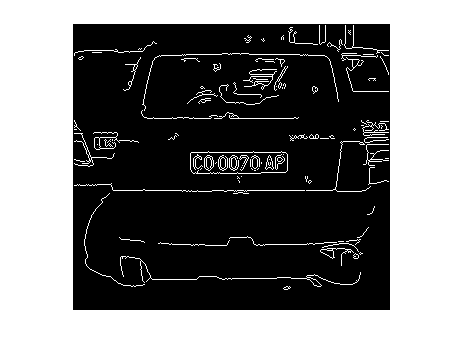
\includegraphics[width=6cm]{sigmabaja.png}}
\subfigure[Sigma Alta.]{
\includegraphics[width=6cm]{sigmaalta.png}}
\caption{\small{Efecto de la modificación del parámetro Sigma.}} \label{Cannysigma}
\end{figure} 

En la imagen (a) se utiliza un valor de \textbf{sigma} muy bajo, por lo que los contornos tienen demasiado detalle. En cambio, en la imagen (b) se ha usado un valor de \textbf{sigma} muy alto, por tanto, el contorno de la matrícula ha perdido su forma original.

\subsection{Búsqueda de las líneas}\label{Hough}
La forma más sencilla de separar la placa de matrícula del resto de la imagen consiste en buscar las dos líneas horizontales que la delimitan usando la transformada de Hough, cuyo funcionamiento se explico en el apartado \ref{hough}\\

En Matlab se implementa la detección de lineas mediante la transformada de Hough con las siguientes funciones:

\begin{lstlisting}
[H, theta, rho] = hough(Img, `Theta', thetaRange,`RhoResolution', rhoResolution);
P  = houghpeaks(H, NumPeaks, 'Threshold', th);
lines = houghlines(Img, theta, rho, P, 'FillGap',maxgap ,'MinLength', lmin);
\end{lstlisting}

Donde:
\begin{itemize}
\item \textbf{thetaRange} es el rango de valores del eje \emph{theta} para los que se buscarán líneas. Para esta aplicación, nos interesa ajustarlo de forma que sólo detecte líneas en dirección horizontal.

\item \textbf{rhoResolution} establece la resolución de la transformada en el eje \emph{rho}. Es decir, controla cuanta variación de \emph{rho} es aceptada en una línea. Para esta aplicación se ha usado $rho~=~7$(píxeles).

\item\textbf{NumPeaks} se corresponde con el máximo número de picos devueltos. En caso de que encuentre más picos que los configurados devolverá los más grandes. En esta aplicación se ha configurado con un número arbitrariamente grande $NumPeaks~=~99$ para tener la certeza de no perder las líneas de la matrícula.

\item\textbf{th} indica el número de líneas que deben coincidir en un punto del plano $\theta\rho$, para ser considerado línea. En esta aplicación se usará el valor por defecto que emplea Matlab $th~=~0.4*max(H)$.

\item\textbf{maxgap} establece la discontinuidad máxima que puede contener una línea para no ser considerada como dos lineas distintas. En esta aplicación se utilizará\\ $maxgap~=~anchoImg/50$.

\item\textbf{lmin} indica la longitud mínima en píxeles que debe tener una línea para ser considerada por el algoritmo. En esta aplicación se emplea $lmin~=~anchoImg/5$.

\item\textbf{H} es una matriz devuelta por la función \emph{hough} que indica el número de líneas que coinciden para cada píxel en el plano~$\theta\rho$. El tamaño de dicha matriz dependerá de la resolución de theta y rho que se haya configurado.

\item\textbf{theta y rho} son los vectores que contienen los ejes theta y rho, usados para crear la matriz \emph{H}.

\item\textbf{P} es la matriz que contiene las coordenadas de cada pico encontrado. Las coordenadas vienen dadas como fila y columna de la matriz \emph{H}.

\item\textbf{lines} es un array de estructuras que contiene la información de cada línea encontrada por la función \emph{houghlines}.
\end{itemize}

La elección de los valores finales se ha determinado, de nuevo, tras realizar pruebas en distintas imágenes; buscando los conjuntos de parámetros que obtengan resultados satisfactorios en la mayoría de ellas. Se entiende por buen resultado la aparición del menor número posible de líneas, pero siempre localizando las de la matrícula. El resultado con los parámetros finales puede observarse en la \reff{Houghfinal}.

\begin{figure}[!h]
\centering
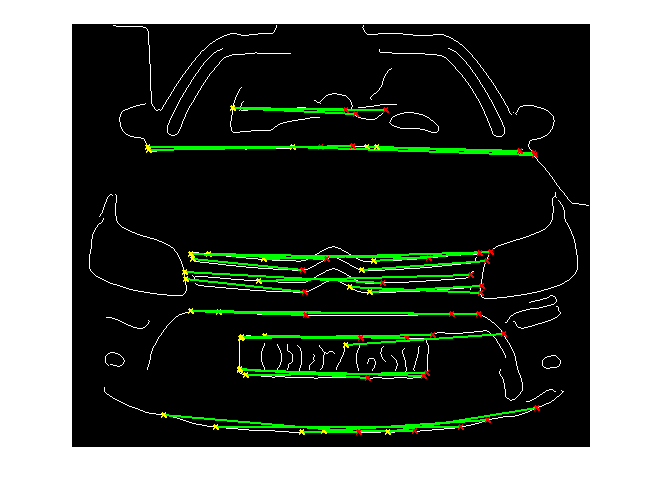
\includegraphics[width=6cm]{EjemploHough.png}
\caption{\small{Detección de líneas con los parámetros seleccionados.}}
\label{Houghfinal}
\end{figure}

A continuación, se estudia el efecto de la variación y el efecto de estos parámetros.\\

Un valor demasiado grande del parámetro rhoResolution provoca que una gran cantidad de líneas sean aceptadas como válidas; mientras que un valor demasiado bajo produciría que no se detectaran las líneas de la matrícula si éstas contienen alguna imperfección. El efecto de la variación del parámetro puede verse en la \reff{cambiorho}. 

\begin{figure}[!h]
\centering \subfigure[Rho Baja.]{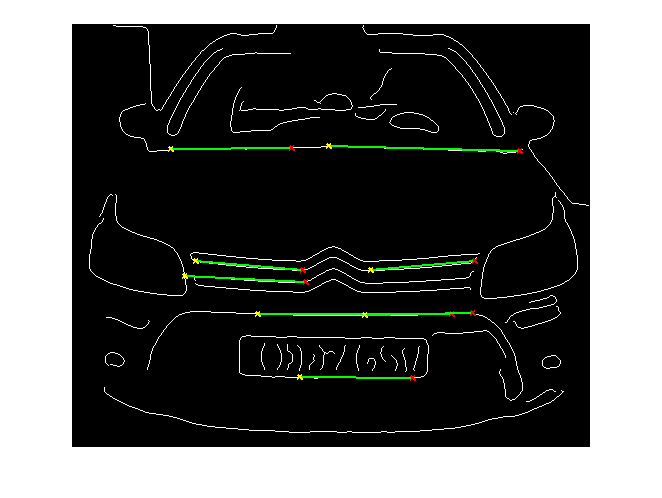
\includegraphics[width=6cm]{rhobaja.png}}
\subfigure[Rho Alta.]{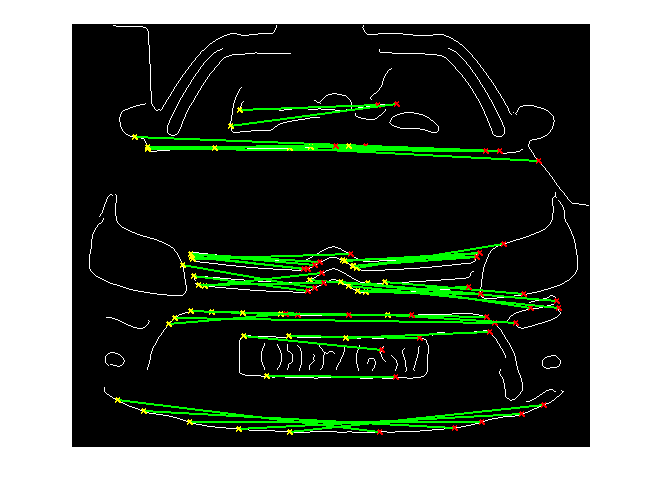
\includegraphics[width=6cm]{rhoalta.png}}
\caption{\small{Efecto de la modificación del parámetro rho.}} \label{cambiorho}
\end{figure} 

La imagen (a) utiliza un valor de rhoResolution demasiado bajo: no se detectan las líneas de la matrícula, ya que no son completamente rectas. Sin embargo, en la imagen (b) se utiliza un valor demasiado alto, lo que resulta en la aparición de un gran número de líneas en la carrocería. Además, al tener tan baja resolución en el eje, no es capaz de diferenciar los píxeles que pertenecen a los contornos de los dígitos de los pertenecientes al borde de la matrícula, lo que produce resultados inesperados. \\

El parámetro \textbf{th} indica lo marcada que debe estar una línea para ser detectada. Se ha optado por dejarlo con el valor por defecto que usa el algoritmo en Matlab.\\

El parámetro \textbf{maxgap} configura la discontinuidad que se considera aceptable en una línea. Un valor demasiado grande produciría la detección de líneas formadas, por píxeles no conectados en absoluto; mientras que un valor muy pequeño ocasionaría la fragmentación de las líneas de la matrícula si contuviesen alguna imperfección. Las consecuencias de la variación de este parámetro pueden apreciarse en la \reff{cambioMaxgap}. 

\begin{figure}[!h]
\centering \subfigure[MaxGap Bajo.]{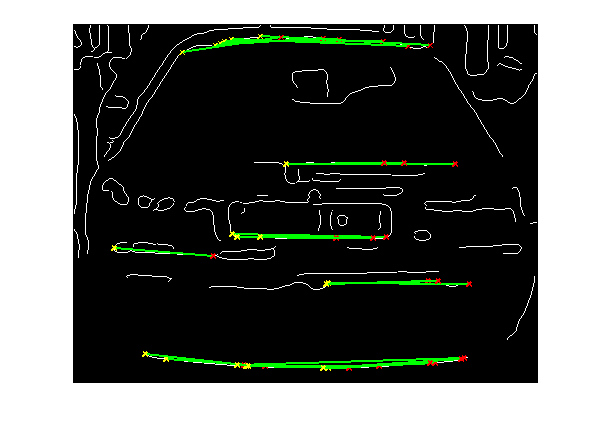
\includegraphics[width=6cm]{gapbajo.png}}
\subfigure[MaxGap Alto.]{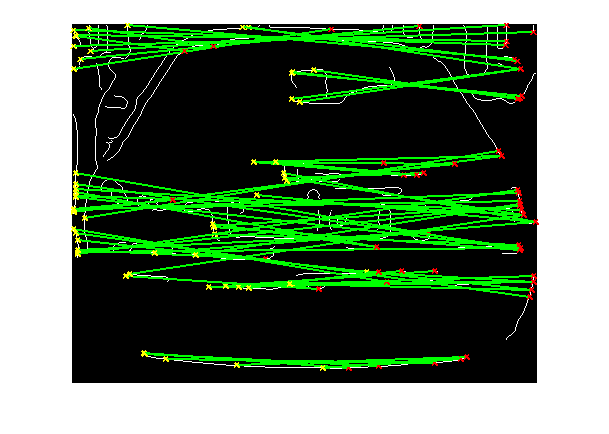
\includegraphics[width=6cm]{gapalto.png}}
\caption{\small{Efecto de la modificación del parámetro MaxGap.}} \label{cambioMaxgap}
\end{figure} 

En la imagen (a) se ha configurado el parámetro con un valor muy bajo, lo que produce que no se detecte la línea superior de la matrícula debido a una imperfección. En la figura (b) se ha configurado con un valor demasiado alto; de ahí la aparición de múltiples líneas surgidas de la conexión de contornos cercanos.  \\

El parámetro \textbf{lmin} es difícilmente configurable sin conocer la localización del sistema que implemente este algoritmo, ya que dependerá en gran medida de la distancia de los vehículos a la cámara que tome las imágenes.


\subsection{Búsqueda del recuadro de la matrícula}
Una vez obtenidas las líneas rectas, es necesario decidir qué par de líneas delimitan el rectángulo. Para ello, buscamos dos líneas que delimiten un rectángulo con las dimensiones aproximadas de una placa de matrícula. Tal y como se muestra en la \reff{dimMat}, las placas de matrícula tienen una dimensión de $520~X~110~mm$; por tanto, sólo nos interesan pares de líneas que tengan un ratio parecido.

\begin{figure}[!h]
\centering
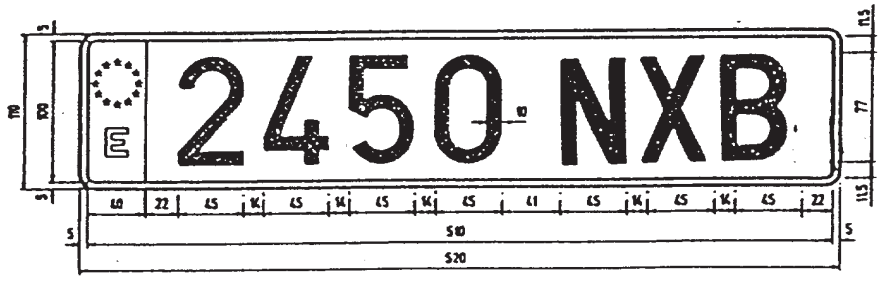
\includegraphics[width=10cm]{boe.png}
\caption{\small{Dimensiones de las placas de matrícula. Fuente:\cite{boe}}}
\label{dimMat}
\end{figure}

El proceso para buscar el rectángulo se describe a continuación:
\begin{enumerate}
\item Se analiza cada pareja de rectas, comprobando si la relación entre la longitud media en el eje x de las dos rectas y la distancia que las separa en el eje y entra en el ratio aceptable.

\item Si la pareja de rectas cumple el ratio se calcula la separación en el eje x de los dos puntos de inicio de las dos rectas, así como la separación entre los dos puntos finales.

\item Elegimos la mayor de las dos distancias calculadas en el punto anterior y la almacenamos en una matriz de distancias.
\end{enumerate}

Una vez completa la matriz distancias, el par de líneas que tenga una distancia menor será el mejor candidato para encontrar la matrícula.

\subsection{Análisis del color del candidato}
Para añadir una mayor probabilidad de acierto, comprobamos que el recuadro que seleccionamos como candidato sea en su mayoría blanco y negro, y que la relación entre píxeles negros y píxeles blancos esté dentro de unos ratios determinados. Esta comprobación ayuda a eliminar rectángulos que aparecen por la forma de la carrocería del coche o debido a alguna sombra; especialmente en coches que no sean de color blanco ni de color negro.\\

Para poder realizar esta segmentación en color se usará la representación LAB en lugar de la clásica RGB. La ventaja que ofrece la codificación LAB es que los colores pálidos están caracterizados por valores pequeños de las magnitudes A y B.

Esto quiere decir que, si se pretende separar los píxeles blancos y negros de aquellos con un color más vivo, sólo debemos aplicar un umbral a dichas magnitudes. Los píxeles que se encuentren por debajo del umbral se considerarán píxeles sin color, es decir, blancos o negros; mientras que los que se encuentren por encima se considerarán píxeles con color. 

Para distinguir píxeles blancos de píxeles negros se debe consultar el valor del parámetro L. Los colores claros se caracterizan por un valor de L bajo, mientras que los colores oscuros tienen valor de L alto.

Por tanto, es necesario establecer otro umbral para este parámetro. Para ello, se ha calculado el Threshold global de la imagen por el método Otsu. De esta forma, se calcula el nivel de gris de la imagen, y se considerarán aquellos píxeles que estén por encima del Threshold como claros y los que estén por debajo como oscuros.\\

Para más información acerca del cálculo del Threshold global con el método Otsu y de su implementación en Matlab, consultar \cite{ImgProcessMat}\\

En la \reff{ModeloLAB} podemos ver una ilustración de la representación LAB.\\

\begin{figure}[!h]
\centering
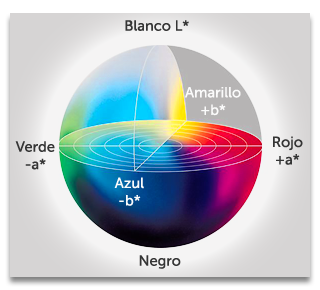
\includegraphics[width=6cm]{LAB.png}
\caption{\small{Ilustración de la representación LAB.}}
\label{ModeloLAB}
\end{figure}

Los umbrales han sido calculados tras realizar pruebas en distintas imágenes, buscando aquellos valores que ofrezcan un mejor resultado en el mayor número de imágenes posibles. Estos valores no han podido ser muy precisos, debido a que dependen en gran medida de la cantidad de píxeles de la carrocería que entren dentro del recuadro de la matrícula.\\

\begin{figure}[!h]
\centering \subfigure[Matrícula bien encuadrada.]{
\includegraphics[width=6cm]{bienEncuadrada.png}}
\subfigure[Matrícula mal encuadrada.]{
\includegraphics[width=6cm]{malEncuadrada.png}}
\caption{\small{Diferencia entre matrículas mal y bien encuadrada.}} \label{DifEncuadre}
\end{figure}

Como podemos ver en la \reff{DifEncuadre}, la imagen (a) está perfectamente encuadrada y no contiene ningún píxel correspondiente al color de la carrocería; mientras que la imagen (b) presenta un encuadre mucho peor con un gran número de píxeles de la carrocería, provocando una significativa variación en la proporción. Por tanto, para evitar que el algoritmo descarte recuadros válidos debido a un mal encuadre, los umbrales deben ser muy generosos.\\

Finalmente, los umbrales elegidos son los siguientes:
\begin{itemize}
\item Píxeles sin color: Coordenadas A y B inferiores a 150
\item Píxeles con color: Coordenadas A y B superiores a 150
\item Píxeles Blancos: Píxeles sin color con coordenada L superior al Threshold
\item Píxeles Negros: Píxeles sin color con coordenada L inferior al Threshold
\end{itemize}


Si el primer candidato cumple con los requisitos de color, será considerado como matrícula. En caso contrario, se seleccionará el segundo candidato con la mejor distancia y se volverá a probar. Este procedimiento se repetirá hasta encontrar una matrícula o hasta que se agoten los candidatos.\\

Para más información sobre el color de imágenes usando coordenadas LAB consultar \cite{matlabLAB}.

\section{Búsqueda de los dígitos}
Para encontrar los dígitos, se convierte la imagen de la matrícula a una representación binaria, donde los píxeles sólo pueden ser blancos o negros. De esta forma, se pueden extraer las distintas figuras de la imagen simplemente buscando conjuntos de píxeles negros aislados. En esta parte del algoritmo, a diferencia de la anterior, se utilizará la imagen original antes del escalado, puesto que resulta más fácil identificar los dígitos si éstos tienen una buena resolución.\\

El diagrama del algoritmo se muestra en la \reff{Diagrama2}.

\begin{figure}[!h]
\centering
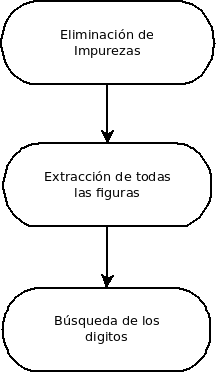
\includegraphics[width=5cm]{Diagrama2.png}
\caption{\small{Diagrama del algoritmo para buscar los dígitos.}}
\label{Diagrama2}
\end{figure}

\subsection{Eliminación de impurezas}
Tras pasar la imagen a representación binaria nos encontramos con pequeñas impurezas que ensucian la imagen y dificultan la detección de los dígitos.\\


Para eliminarlas hay que establecer un área mínima y borrar todos los conjuntos de píxeles que tengan un área menor a la establecida. Esto se puede llevar a cabo mediante la siguiente función de Matlab:

\begin{lstlisting}
matriculaSinImpurezas = not bwareaopen( not matriculaConImpurezas, areaMin)
\end{lstlisting}


Donde \textbf{areaMin} es el área mínima que deben tener los conjuntos de píxeles para no ser eliminados. Se ha establecido \textbf{areaMin} como un 5\% del área total de la matrícula.\\

Como se puede ver en la función tanto la imagen origen como el resultado de la función están negados. Esto se debe a que la función entiende por píxel activo un píxel blanco, mientras que en nuestra aplicación consideramos como píxeles activos a los píxeles negros.\\

Los resultados pueden apreciarse en la \reff{Impurezas}

\begin{figure}[!h]
\centering \subfigure[Matrícula con impurezas.]{
\includegraphics[width=6cm]{MatriculaImpurezas.png}}
\subfigure[Matrícula sin impurezas.]{
\includegraphics[width=6cm]{MatriculaSinImpurezas.png}}
\caption{\small{Resultado de la eliminación de impurezas.}} \label{Impurezas}
\end{figure}

\subsection{Extracción de todas las figuras}
El siguiente paso es identificar y extraer todas las figuras de la imagen, entre las que se encuentran los dígitos que forman el número de matrícula.

\newpage 
Extraemos las figuras con el siguiente código de Matlab:

\begin{lstlisting}
[Figuras Ne]=bwlabel( not matricula);
for n=1:Ne
	[h,w] = find(Figuras==n);
	fig(i)=matricula(min(h):max(h),min(w):max(w));
end
\end{lstlisting}

Donde:\begin{itemize}
\item \textbf{Figuras} es una matriz donde las posiciones correspondientes a los píxeles de cada una de las figuras tienen como valor un número entero distinto; mientras que los que pertenecen al fondo están marcados como 0.

\item \textbf{Ne} es el número de figuras encontradas.

\item\textbf{h} y \textbf{w} son dos variables auxiliares donde se almacenan las dimensiones de la figura encontrada.

\item\textbf{fig} es un vector donde guardan todos los resultados.
\end{itemize}

Entre las figuras encontradas, los dígitos de la matrícula no son los únicos resultados que aparecen. También se encuentras otras figuras pertenecientes a la carrocería del coche, o el símbolo de la Unión Europea, que deben ser filtrados.\\

En la \reff{Figuras} se pueden observar dos de los objetos extraídos de la matrícula representada en la \reff{Impurezas}. La imagen (a) representa un trozo del símbolo de la Unión Europea. La imagen (b) muestra uno de los números de la matrícula. Para esta aplicación, el símbolo de la Unión Europea carece de interés; por tanto, debemos ignorarlo mientras que el dígito sí debe ser procesado.

\begin{figure}[!h]
\centering \subfigure[Figura no deseada.]{
\includegraphics[width=5cm]{figuraBasura.png}}
\subfigure[Dígito de la matrícula.]{
\includegraphics[width=5cm]{figuraBuena.png}}
\caption{\small{Algunas de las figuras extraídas de la matrícula.}} \label{Figuras}
\end{figure}

\subsection{Búsqueda de los dígitos}
Por último, el algoritmo debe decidir qué resultados se corresponden con un dígito y qué resultados no. Para ello, se analizan las características de todas las figuras encontradas y se comparan con las que habitualmente se encuentran en la tipografía utilizada.\\

Las características analizadas son el área de la figura, la relación entre el alto y el ancho de la figura, la relación entre el número de píxeles blancos y negros y el número de píxeles negros.\\

Los valores de los umbrales se han decidido calculando las máximas variaciones de las características analizadas en la tipografía presente en las matrículas.\\

Pero el desgaste de las matrículas y los errores en las imágenes, tales como la inclinación o una mala iluminación, añaden imperfecciones a los dígitos extraídos. Por este motivo, ha sido necesario sumar un margen de error a los umbrales calculados. Este margen de error se ha calculado tras realizar pruebas en distintas imágenes.\\

Los umbrales resultantes son los siguientes:

\begin{itemize}
\item Área de la figura inferior al 30\% del área de la matrícula. 
\item Relación entre el alto y el ancho de la figura entre 8 y 1,3.
\item Relación entre el número de píxeles blancos y negros inferior a 4.
\item Número de píxeles negros superior a 0,4 multiplicado por la media de píxeles negros en las figuras encontradas, e inferior a 1,8 multiplicado por la media.
\end{itemize}

Las figuras que cumplan los requisitos serán consideradas como dígitos de la matrícula.\\

Un problema encontrado es que, a pesar de intentar ajustar los umbrales lo máximo posible, la figura de la Unión Europea habitualmente es reconocido como carácter válido y posteriormente identificado como una la letra `I'. Para solucionar este problema sería necesario un análisis del color de las figuras encontradas y eliminar aquellas que no sean negras.

\section{Decisión del número de matrícula}
La última tarea que debe realizar el algoritmo \ac{ALPR} es decidir con qué carácter se corresponde cada uno de los dígitos encontrados en la etapa anterior.\\

Para ello, el programa almacenará una base de datos con las imágenes de cada uno de los dígitos que componen la tipografía empleada en las matrículas. De esta forma, sólo hay que comparar cada uno de los dígitos encontrados en la imagen con cada dígito de la tipografía, y elegir aquel que nos dé una coincidencia más alta.\\

Para realizar la comparación se escalan las imágenes de forman que tengan el mismo tamaño y comprobamos píxel a píxel.\\

\begin{figure}[!h]
\centering \subfigure[Dígito encontrado.]{
\includegraphics[width=5cm]{9.png}}
\subfigure[Dígito de la tipografía.]{
\includegraphics[width=5cm]{A.png}}
\subfigure[Resultado de la comparación.]{
\includegraphics[width=5cm]{ComparacionA_9.png}}
\caption{\small{Ejemplo de comparación erronea.}} \label{ComError}
\end{figure}

En la \reff{ComError} se puede observar el resultado de una comparación errónea. La figura (a) se corresponde con un dígito encontrado en la imagen, mientras que la figura (b) es un carácter de la tipografía. El resultado de la comparación se muestra en la figura (c). \\

Los píxeles blancos se corresponden con los píxeles que coinciden en las dos imágenes, y los negros con los que no. Puesto que no se trata del mismo dígito, el resultado de la comparación es malo.\\

En la \reff{ComCorrecta} se puede ver un ejemplo de una comparación correcta: en esta ocasión el dígito encontrado en la figura y el de la tipografía son el mismo, por tanto, la mayoría de los píxeles coinciden.

\begin{figure}[!h]
\centering \subfigure[Dígito encontrado.]{
\includegraphics[width=5cm]{9.png}}
\subfigure[Dígito de la tipografía.]{
\includegraphics[width=5cm]{9_tipografia.png}}
\subfigure[Resultado de la comparación.]{
\includegraphics[width=5cm]{Comparacion9_9.png}}
\caption{\small{Ejemplo de comparación correcta.}} \label{ComCorrecta}
\end{figure}



% ------------------------------------------------------------------------
%                             Capítulo 4
% ------------------------------------------------------------------------
\chapter{Implementación en C++}

Este capítulo trata el proceso de traducción del código de Matlab a C++ mediante las funciones de la librería gráfica OpenCV. La mayor parte del trabajo es una traducción directa, debido a que la mayoría de las funciones utilizadas en Matlab tienen un equivalente en OpenCV. 

Una explicación detallada del proceso consistiría esencialmente en volver sobre lo tratado en el capítulo anterior. Por tanto este capítulo sé centrará en las mayores diferencias entre las dos implementaciones; así como los problemas encontrados en el proceso.

\section{Algoritmo de Canny}
La primera diferencia reside en el algoritmo de Canny. La implementación y la parametrización que utiliza OpenCV es diferente a la que utiliza Matlab. Además, la rutina de Matlab implementa el filtrado gaussiano en la misma rutina que el algoritmo de Canny; mientras que en OpenCV es necesario utilizar dos rutinas diferentes.\\

\begin{figure}[!h]
\centering 
\subfigure[Matlab]{
\includegraphics[width=6cm]{EjemploCanny.png}}
\subfigure[OpenCV]{
\includegraphics[width=6cm]{CannyOpenCV1.png}}
\caption{\small{Resultado del algoritmo con los mismos parámetros.}} \label{CannyOpenCV}
\end{figure}

En la \reff{CannyOpenCV} pueden observarse los diferentes resultados que produce el algoritmo de Canny en Matlab y OpenCV usando los mismos parámetros. La imagen (a) muestra el resultado del algoritmo de Canny en Matlab, tal y como se vio en \ref{Canny}; mientras que en la imagen (b) se observa el resultado del algoritmo en OpenCV utilizando los mismos parámetros.\\


Resulta evidente que este resultado no es aceptable, por lo que es necesario volver a calcular los parámetros del algoritmo.\\

Durante este proceso de parametrización se llegó a la conclusión de que se pueden conseguir resultados interesantes utilizando diferentes valores de desviación típica en el filtro gausiano para los ejes $x$ e $y$, lo cual es posible gracias a que la rutina de filtro gausiano utilizada en OpenCV lo permite.\\


\begin{figure}[!h]
\centering 
\subfigure[Misma desviación típica.]{
\includegraphics[width=6cm]{CannyOpenCV2.png}}
\subfigure[Distinta desviación típica.]{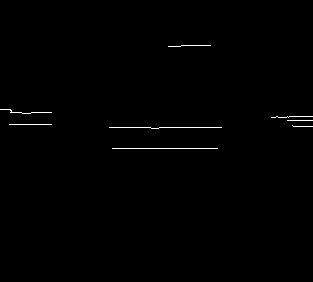
\includegraphics[width=6cm]{CannyOpenCV3.png}}
\caption{\small{Efecto de usar distintas desviaciones tipicas en los ejes.}} \label{CannyOpenCV2}
\end{figure}

En la \reff{CannyOpenCV2}, se observa un ejemplo de esta idea. La imagen (a) representa el resultado del algoritmo de Canny, donde se ha empleado la misma desviación típica en los dos ejes y una parametrización que consigue resultados similares a los obtenidos con Matlab en el apartado \ref{Canny}. La imagen (b) muestra el resultado tras aplicar una desviación típica mayor en el eje $x$ que en el $y$. \\

Lo que ocurre en la imagen (b) se debe a que el filtro distorsiona completamente los contornos verticales, dejando los horizontales intactos. Esto simplifica enormemente el trabajo de encontrar las líneas de la matrícula, ya que los candidatos a matrícula se reducen en gran medida.\\

El código C++ utilizado para realizar el algoritmo es el siguiente:

\begin{lstlisting}
GaussianBlur( ImgOriginal, ImgFiltrada, DimFiltro, sigmax, sigmay);
Canny(ImgFiltrada, ImgContornos, T1, T2);
\end{lstlisting}

Donde:
\begin{itemize}
\item \textbf{DimFiltro} es el parámetro que configura la dimensión del kernel usado por el filtro. En esta aplicación se ha configurado con tamaño 0 para que la función decida el tamaño.
\item \textbf{sigmax y sigmay} se corresponden con las desviaciones típicas usadas en los ejes $x$ e $y$ respectivamente. En esta aplicación se configuran con $sigmax=10$ y \\$ sigmay=1$.
\item\textbf {T1 y T2} se corresponden con los umbrales usados por el algoritmo para determinar los contornos. En esta aplicación se eligen como valores $T1=100$ y $T2=250$.
\end{itemize}

\section{Transformada de Hough}\label{CannyCV}
Otra diferencia la encontramos en la transformada de Hough.\\

OpenCV cuenta con una función que busca directamente las líneas rectas en una imagen usando la transformada de Hough:


\begin{lstlisting}
HoughLinesP(ImgContornos, lines, rho, theta, th, minLength, maxGap );
\end{lstlisting}

Donde:
\begin{itemize}
\item \textbf{lines} es una estructura donde se almacenan las líneas encontradas.

\item \textbf{rho y theta} se corresponden con la sensibilidad usada en los eje rho y theta para calcular las líneas. En esta aplicación se configuran como $tho=w/300$ (píxeles) y $ theta=1º$.

\item\textbf {th} indica el número de líneas que deben coincidir en un punto en el plano $ab$ para ser considerado línea. En esta aplicación se usará $th = anchoImg/10$.

\item\textbf{minLength} indica la longitud mínima en píxeles que debe tener una línea para ser considerada. Para esta aplicación se usará $minLength~=~anchoImg/5$.

\item\textbf{maxGap} establece la discontinuidad máxima que puede contener una línea para que no sea considerada como dos líneas distintas. En esta aplicación se utilizara\\ $maxGap~=~anchoImg/10$.
\end{itemize}

En el parámetro \textbf {th} se halla la primera diferencia respecto a Matlab. En la implementación en Matlab se tiene acceso directo a la matriz \textbf{H}, como se vio en el apartado \ref{Hough}, lo que hace posible configurar \textbf {th} en función del máximo de \textbf{H}.\\

Otro problema encontrado es el que se ilustra en la \reff{ProblemaLineasOpenCV}.\\

\begin{figure}[!h]
\centering \subfigure[Resultado del algoritmo de Canny.]{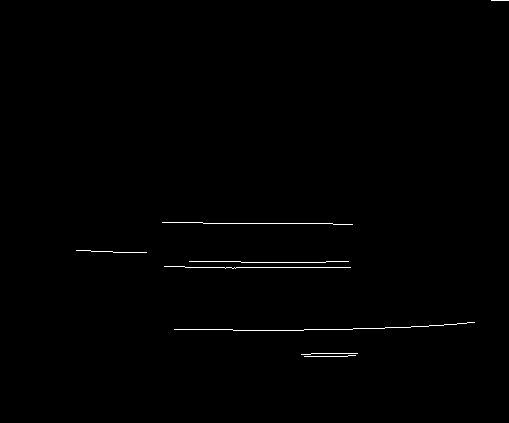
\includegraphics[width=6cm]{ProblemaCannyOpenCV.png}}
\subfigure[Líneas encontradas.]{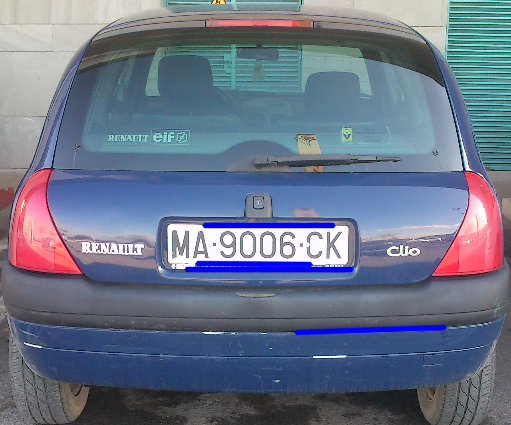
\includegraphics[width=6cm]{ProblemaLineasOpenCV.png}}
\caption{\small{Problemas con la detección de líneas.}} \label{ProblemaLineasOpenCV}
\end{figure}

La imagen (a) muestra el resultado del algoritmo de Canny, donde se muestran todos los contornos detectados en la imagen. Entre ellos se encuentran los dos contornos correspondientes a la matrícula con pequeñas imperfecciones. En la imagen (b) se observan las líneas encontradas por la función. Puede observarse cómo el algoritmo no ha reconocido la línea completa debido a las imperfecciones.\\

La solución a este problema consiste en reducir la sensibilidad usada por el algoritmo mediante los parámetros \textbf{rho} y \textbf{theta}; pero el resultado obtenido no se corresponde con el esperado. La reducción de la sensibilidad no produce ninguna mejora en absoluto, y no se ha encontrado ninguna combinación de parámetros que consiga solucionar el problema.\\

Encontrar una solución definitiva para el problema pasa por investigar la implemtentación que realiza OpenCV de la transformada de Hought, para modificarla o realizar pruebas con otras funciones de transformada de Hough disponibles de forma libre. No obstante, la duración de este \ac{TFG} no permite la realización de estas pruebas.
% ------------------------------------------------------------------------
%                             Capítulo 5
% ------------------------------------------------------------------------
\chapter{Conclusiones y líneas futuras}
Para finalizar en este capítulo se analizan las conclusiones extraídas de la realización de este \ac{TFG}, así como algunas de las posibles líneas a seguir para mejorar el trabajo realizado.

\section{Conclusiones}
El objetivo de este \ac{TFG} era el desarrollo de un algoritmo \ac{ALPR} básico con vistas a su implementación en una placa Raspberry Pi.\\

Para llevarlo a cabo, en primer lugar se ha realizado un modelo inicial del algoritmo usando el entorno Matlab. Se ha preferido realizar este primer paso en lugar de proceder directamente a la implementación en C++ ya que Matlab ofrece una gran facilidad para depurar código; siendo posible detener la ejecución del código en cualquier punto, acceder al valor de las variables e incluso realizar operaciones con estos valores. Además, la forma de representación de las imágenes que usa resulta muy cómoda para depurar el algoritmo; puesto que es posible tratar la imagen tanto con funciones de alto nivel como acceder al valor individual de cada píxel.\\

Como contrapartida, el desarrollo en C++ no cuenta con tantas facilidades.  Pero en cambio, produce un código mucho más rápido y fácilmente portable a un gran número de dispositivos.\\

En cuanto al algoritmo \ac{ALPR}, la combinación de la función Canny con la transformada de Hough ha demostrado dar buenos resultados a la hora de detectar las placas de matrícula; especialmente cuando las imágenes son tomadas en buenas condiciones de luminosidad.\\

Otra conclusión obtenida es que el método utilizado para calcular la correlación entre los dígitos extraídos de  la imagen y los dígitos de la tipografía no es lo suficientemente eficaz. Durante la realización de este TFG se ha empleado un método basado en la comparación píxel a píxel. Esto provoca numerosos errores, especialmente si la matrícula presenta daños. También se han encontrado problemas con el carácter de la Unión Europea, presente en la mayoría de las matrículas, puesto que lo reconoce como un carácter válido.\\

Por último, se ha podido comprobar la importancia de la iluminación en este tipo de algoritmos. Una aplicación \ac{ALPR} comercial debería encontrar alguna forma de controlar este factor.

\section{Líneas futuras}
A continuación se presentan algunas posibles vías para completar y mejorar el trabajo presentado:

\begin{itemize}
\item Completar la implementación en C++/OpenCV. La segmentación en color no pudo ser implementada en OpenCV debido a limitaciones de tiempo. Por tanto, es la línea de continuación más clara. Además, como se explico en el apartado \ref{CannyCV}, la función que realiza la detección de las líneas mediante la transformada de Hough debe ser revisada.

\item Ejecutar el algoritmo sobre la placa Raspberry Pi. Una vez se cuenta con el código en C++/OpenCV es necesario utilizar un compilador cruzado para generar un ejecutable que pueda funcionar sobre la placa. También habría que desarrollar el código necesario para utilizar la cámara disponible en la placa como fuente de las imágenes.

\item Estudiar la posibilidad de hacer compatible el algoritmo desarrollado con otros sistemas. Resultaría especialmente interesante una versión compatible con smartphones, debido a su gran éxito comercial y a que generalmente disponen de cámara de vídeo y potencia de cómputo suficiente para ejecutar un algoritmo \ac{ALPR}.
\end{itemize}

%Cambia el Título Capítulo por Apéndice (no lo hará automáticamente con \appendix porque se forzo la definición de Capítulo en config.tex)
\titleformat{\chapter}[hang]{\Huge\bfseries}{\fontsize{24}{60} Apéndice \thechapter{. }}{0pt}{\fontsize{24}{60}}
\appendix

%\input{Apendice_A.tex}
%\input{Apendice_B.tex}

\cleardoublepage

\addcontentsline{toc}{chapter} {Referencias}
\label{Referencias}


\renewcommand\bibname{Referencias}
\bibliography{bibliografia} 
\bibliographystyle{IEEEtran}  %con numeros
%\bibliographystyle{IEEEpes}  %con numeros
%\bibliographystyle{amsalpha}  %con abreviaturas
%\bibliographystyle{apalike} %con el nombre entero autor + fecha, problema orden nombres

\end{document}
